\documentclass[11pt,letter]{article}
\usepackage[top=1.00in, bottom=1.0in, left=1.1in, right=1.1in]{geometry}
\renewcommand{\baselinestretch}{1.1}
\usepackage{graphicx}
\usepackage{natbib}
\usepackage{amsmath}
\usepackage{amssymb} 
\usepackage{hyperref} 

\def\labelitemi{--}
\parindent=0pt
\begin{document}

% \bibliographystyle{..//..//refs/bibstyles/Science.bst}

\title{Sensitivities are not declining with warming} 
\author{E. M. Wolkovich$^{1,2,3,a}$, C. J. Chamberlain$^{1,2}$, D. M. Buonaiuto$^{1,2}$, \\ A. K. Ettinger$^1$, I. Morales-Castilla$^{1,2,4}$}

\date{\today} 
\maketitle
$^1$Arnold Arboretum of Harvard University, Boston, Massachusetts 02131, USA\\
$^2$Department of Organismic and Evolutionary Biology, Harvard University, Cambridge, Massachusetts, USA\\
$^3$Forest \& Conservation Sciences, Faculty of Forestry, University of British Columbia, Vancouver, British Columbia, Canada\\
$^4$Department of Life Sciences, University of Alcal\`a CTRA N-II, KM., 33,600, 28802, Alcal\`a de Henares, Spain\\
$^a$Corresponding author.

\section{Outline \& notes}

Need to work on this, notes to date on \href{https://github.com/lizzieinvancouver/ospree/wiki/Statistical-artifacts-in-sensitivities}{here}

\section{Tasks, milestones etc.}
\begin{itemize}
\item Finish minimal analyses we think we need:
\begin{itemize}
\item Produce simulated data where chilling is not met (Lizzie has notes on this below enddocument command ... (bucket model).
\item Do sliding windows for ... BETPEN (done) and FAGSYL from PEP725 and for simulated data.
\end{itemize}
\item Review the literature
\begin{itemize}
\item Cat did some of this [add LINK HERE]
\item Review beyond phenology?
\end{itemize}
\item Outline the paper
\item Decide on targeted journals
\item Write the paper
\item Submit the paper
\end{itemize}



\section* {Figures}

\begin{figure}[h!]
\centering
\noindent 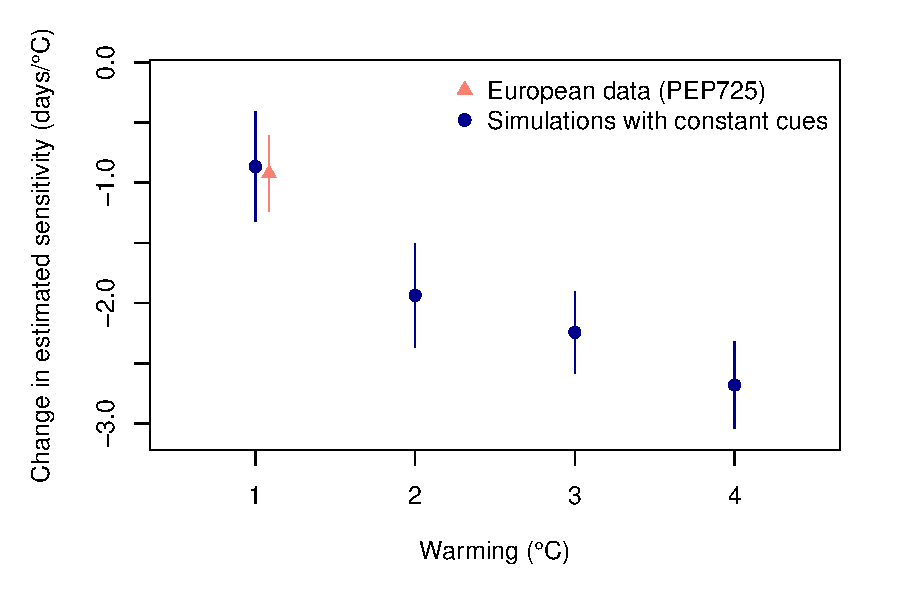
\includegraphics[width=0.75\textwidth]{..//..//analyses/bb_analysis/PEP_climate/figures/peprealandsims.pdf}
\caption{\textbf{Declining sensitivities observed in long-term European data for a suite of common trees may be explained by a statistical artifact.} We compared the sensitivity estimated from linear regressions of day of leafout versus mean spring temperature (estimated thus as days/$^{\circ}$C) from PEP725 data for \emph{Betula pendula} from 45 sites (``European data'') with estimated declines in simulations where the cues were held constant but spring temperatures warmed by 1-4$^{\circ}$C (``Simulations'') and found the estimated temperature sensitivity measured as days/$^{\circ}$C declined even though the underlying cues had not changed, see \emph{Understanding declines in temperature sensitivity in European long-term data} for further details.}
\label{fig:pepsims}
\end{figure}

\end{document}

Simulate bucket model task

Weather first (1-5), then phenology (6-7):
1. Skip fall
2. Simulate stochastic stationary, cold winter (make sure this hits too little chill at some level of warming)
3. Simulate stochastic stationary, warm spring
4. Build transition between 3 and 4.
5. Do warming as we have -- add 1:7 degrees
6. Calculate GDD (1 Jan onward) and chilling (1 Nov - 1 Feb)
7. Select some range of high chill where same GDD is needed for budburst, then set up a linear relationship between chill (at lower range) and GDD required (more GDD for lower chill)
8. Predict GDD based on simulated weather and 7.

\begin{align*}
y_i &= \alpha_{sp[i]} + \beta_{forcing_{sp[i]}} + \beta_{photoperiod_{sp[i]}} + \beta_{chilling_{sp[i]}} + \beta_{latitude_{sp[i]}} + \beta_{photoperiod x latitude_{sp[i]}} + \epsilon{_i},\\
\epsilon_i \sim N(0,\sigma^2_y)
\end{align*}

This would be better .., 

\begin{align*}
y_i &= \alpha_{sp[i]} + \beta_{forcing_{sp[i]}} + \beta_{photoperiod_{sp[i]}} + \beta_{chilling_{sp[i]}} + \beta_{latitude_{sp[i]}} + \beta_{photoperiod x latitude_{sp[i]}} + \epsilon{_i},\\
& \epsilon_i \sim N(0,\sigma^2_y)
\end{align*}

or ...

\begin{align*}
y_i &= \alpha_{sp[i]} + \beta_{forcing_{sp[i]}} + \beta_{photoperiod_{sp[i]}} + \beta_{chilling_{sp[i]}} + \\
& \beta_{latitude_{sp[i]}} + \beta_{photoperiod x latitude_{sp[i]}} + \epsilon{_i}, \epsilon_i \sim N(0,\sigma^2_y)
\end{align*}


% \bibliography{..//..//refs/ospreebibplus.bib}
